% mnras_template.tex 
%
% LaTeX template for creating an MNRAS paper
%
% v3.0 released 14 May 2015
% (version numbers match those of mnras.cls)
%
% Copyright (C) Royal Astronomical Society 2015
% Authors:
% Keith T. Smith (Royal Astronomical Society)

% Change log
%
% v3.0 May 2015
%    Renamed to match the new package name
%    Version number matches mnras.cls
%    A few minor tweaks to wording
%    
%    Beta testing only - never publicly released
%    First version: a simple (ish) template for creating an MNRAS paper

%%%%%%%%%%%%%%%%%%%%%%%%%%%%%%%%%%%%%%%%%%%%%%%%%%

\documentclass[usenatbib]{mnras}

%\usepackage{newtxtext,newtxmath}
\usepackage[T1]{fontenc}


%%%%% AUTHORS - PLACE YOUR OWN PACKAGES HERE %%%%%
\usepackage{graphicx}	% Including figure files
\usepackage{amsmath}	% Advanced maths commands
\usepackage{amssymb}	% Extra maths symbols

%%%%%%%%%%%%%%%%%%%%%%%%%%%%%%%%%%%%%%%%%%%%%%%%%%

%%%%% AUTHORS - PLACE YOUR OWN COMMANDS HERE %%%%%


\newcommand{\vdag}{(v)^\dagger}
\newcommand\aastex{AAS\TeX}
\newcommand\latex{La\TeX}
\newcommand{\Msun}{\,{\rm M}$_{\odot}$\,}
\newcommand{\kms}{\,{\rm km s}\ifmmode ^{-1}\,\else $^{-1}$\,\fi}
\newcommand{\Mpch}{\,{\rm Mpc}\,\ifmmode h^{-1}\else $h^{-1}$\fi}
\newcommand{\kpch}{\,{\rm kpc}\,\ifmmode h^{-1}\else $h^{-1}$\fi}
\newcommand{\kpc}{\,{\rm kpc}\,}

%%%%%%%%%%%%%%%%%%%%%%%%%%%%%%%%%%%%%%%%%%%%%%%%%%
\title[The $\beta$-skeleton and the T-web]{Cosmic web classification of galaxies from the $\beta$-skeleton}

% The list of authors, and the short list which is used in the headers.
% If you need two or more lines of authors, add an extra line using \newauthor
\author[J. F. Su\'arez-P\'erez et al.]{
J. F. Su\'arez-P\'erez,$^{1}$\thanks{E-mail: jf.suarez@uniandes.edu.co}
Y. Camargo,$^{2}$ 
X.-D. Li,$^{3}$
and J. E. Forero-Romero,$^{1}$
\\
% List of institutions
$^{1}$Departamento de F\'isica, Universidad de los Andes, Cra. 1 No. 18A-10 Edificio Ip, CP 111711, Bogot\'a, Colombia\\
$^{2}$Departamento de F\'isica, Universidad Nacional de Colombia, Ciudad Universitaria, Bogot\'a, Colombia\\
$^{3}$School of Physics and Astronomy, Sun Yat-Sen University, Guangzhou 510297, P.R.China\\
}

% These dates will be filled out by the publisher
\date{Accepted XXX. Received YYY; in original form ZZZ}

% Enter the current year, for the copyright statements etc.
\pubyear{2020}

% Don't change these lines
\begin{document}
\label{firstpage}
\pagerange{\pageref{firstpage}--\pageref{lastpage}}
\maketitle

% Abstract of the paper
\begin{abstract}
We show how it is possible to infer the environments of the cosmic web
of dark matter using the information of the spatial distribution of
galaxies and a machine learning algorithm.
Handled the set of galaxies
as a set of nodes, we applied the $\beta$-skeleton algorithm to
extract geometrical information like the number of connections or the
average distance by galaxy.
Using this properties of the distribution
of galaxies was probed the classification trees, random forest and SVM algorithms under
different configurations to find the best set of parameters that makes
a good prediction with the lowest confusion. 
The results show that the
local average distance between galaxies on the $\beta$-skeleton is the
most important feature for the prediction of the cosmic web
environment. 
This is a good approximation that will allow us to use
these algorithms to make predictions in observational data. 
\end{abstract}

% Select between one and six entries from the list of approved keywords.
% Don't make up new ones.
\begin{keywords}
cosmic web -- $\beta$-skeleton -- machine learning
\end{keywords}

%%%%%%%%%%%%%%%%%%%%%%%%%%%%%%%%%%%%%%%%%%%%%%%%%%

%%%%%%%%%%%%%%%%% BODY OF PAPER %%%%%%%%%%%%%%%%%%
\section{Introduction}
The galaxy distribution on large spatial scales follows a structured 
pattern commonly know as the cosmic web. 
This web consists of dense spherical peaks connected by
anisotropic filaments and walls woven across vast under-dense voids.
\citep{Bond1996}. 
Such a structure can also be interpreted in the context of 
the evolution from initial density fluctuations to the present-day 
large-scale structure within a $\Lambda$CDM cosmology \citep{ZelDovich1970,White1987}. 
The cosmic web emergence can be followed in great detail by studying DM only
cosmological simulations.
There is a great variety of methods to detect and classify regions of
space as belonging to a peak, filament, sheet or void
\citep{Libeskind2018}.

However, the cosmic web recognition algorithms that seek to work
directly on the discrete galaxy distribution are less abundant.
There are specific algorithms that can be used to find voids \citep{Platen2007,Neyrinck2008,Ravoux2020}, filaments \citep{Novikov2003,Zhang2009,Sousbie2010,Chen2015,Luber2019,Malavasi2020}, filaments and sheets \citep{Zhang2009}, peaks,filaments and sheets \citep{Aragon-Calvo2019} or peaks,filaments and voids \citep{Buncher2019}, 
but a generic approach to predict the full cosmic web environments 
from the galaxy distribution relies either on performing 
the reconstruction of the dark matter around the galaxies
or using an approximation where galaxies are interpolated over a 
grid to process them in the same way as dark matter densities.

Many dark matter reconstruction methods use Bayesian statistics
coupled with Monte Carlo sampling
\citep{Jasche2010,Jasche2013a,Bos2014,LeclercqJasche2015,Horowitz2019,Burchett2020}. Other methods reconstruct the cosmic density field from the distribution of dark matter halos \citep{Wang2009}. In contrast some procedures emulate the dark matter density field with a matter 
overdensity field reconstructed from the distribution of galaxies with 
mechanism like the Delaunay Tessellation Field Estimator (DTFE),
a reconstruction methodology to the sample particle or galaxy 
distribution  \citep{Schaap2007,Platen2011,Aragon-Calvo2007,Aragon-Calvo2010,Cautun2013,Cautun2014}, 
then this overdensity field is used jointly with other algorithms or methodologies to make the classification by environments of the cosmic web. Recently, other procedures compute different properties of dark matter halos and make the classification using these input with machine learning methods \citep{Hui2018}. 
Either way, dark matter reconstruction remains computationally expensive task. 

Other methodologies to make the environments classification compute some features directly on the galaxies. The galaxy clustering and quenching are quantified in terms of the spherical overdensity $\delta_8$ and the tidal anisotropy $\sigma_5$ \citep{Shadab2019}. In \citep{Eardley2015} are estimated the  tidal  tensor  from  a smoothed galaxy overdensity field in order to determine the dimensionality of collapse of any region. Other works study the influence of some features of the galaxies like the colour, brightness, morhological properties, gas metallicity, and total spectral energy density in the large scale structure \citep{Alpaslan2016}. Also, some properties like the normalized stellar mass and the local overdensity $\delta_4$ are used to make the classification \citep{Tojeiro2017}. In \citep{Horowitz2019} is reconstructed the initial density field from Lyman-$\alpha$ datasets to infer the underlying matter density and make the classification by environments.

The goal of this paper is to avoid expensive reconstruction algorithms
and binning of galaxy data to provide a new way to connect the galaxy
distribution to its dark matter web environment.
To do that, we build a graph on top of the galaxy distribution 
to build a set of features that can be used to predict the web
environment.

We demonstrate an specific implementation of this approach using 
the $\beta$-skeleton graph \citep{Fang2019} and the 
T-web \citep{Forero-Romero2009} cosmic web classification.
We test three different supervised machine learning
algorithms (support vector machine, Tree Classifier, Random Forest) 
to train from the features and predict the environment.
We quantify the precision and accuracy of the algorithms using 
the Illustris-TNG simulation \citep{Nelson2015} at redshift $z=0$.

This paper is organized as follows. 
In section \ref{sec:init} we describe the T-web algorithm,
the $\beta$-skeleton graph and the summarize the most important
aspects of the Illustris-TNG simulations relevant to our work.
In the section \ref{sec:link} we
describe the mechanism to link the $\beta$-skeleton to the T-Web
using machine learning algorithms. 
There we detail the features and meta-parameters we use, the
classification algorithms and the metrics for model evaluation 
In the section \ref{sec:results} we present our results
to finally summarize our conclusions in \ref{sec:conclusions}.


\section{Initial Algorithms and Simulations}\label{sec:init}

\begin{figure*}
\centering
 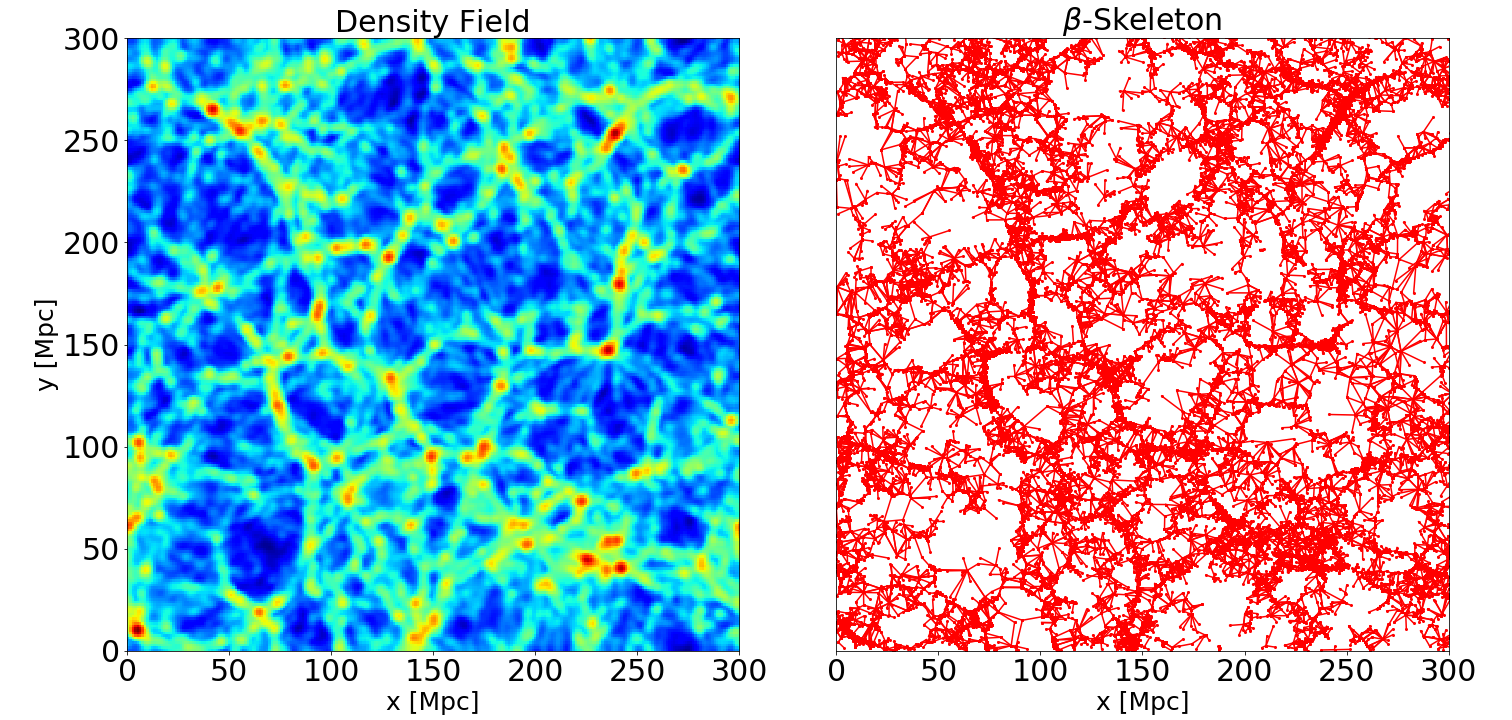
\includegraphics[scale=0.3]{Figs/Fig1_.png}
 \caption{Comparison between the T-Web of dark matter density field (left) and the $\beta$-skeleton (right) computed from the distribution of galaxies with $\beta$=1 for Illustris-TNG300.}
 \label{fig:Fig1}
\end{figure*}



\subsection{T-Web Classification}

The tidal web (T-Web) method \citep{Hahn2007,Forero-Romero2009} classifies the large scale
structure into four web types: voids, sheets, filaments and peaks. 
This classification is based on the eigenvalues of the deformation tensor $T_{\alpha\beta}$, the Hessian of the gravitational potential
\begin{equation}
T_{\alpha\beta}=\frac{\partial^2\psi}{\partial r_{\alpha}r_{\beta}},
\end{equation}
%
where $\psi$ is a normalized gravitational potential that follows the equation
\begin{equation}
    \nabla^2 \psi = \delta,
\end{equation}
%
and $\delta$ is the dark matter overdensity.
This tensor has three real valued eigenvalues. 
The cosmic web environment is defined by the number of eigenvalues larger than
a threshold value $\lambda_{th}$.
Locations with three eigenvalues larger than $\lambda_{th}$ correspond to a peak, two to a filament, one to a sheet and zero to a void.

Computationally speaking, to define an environment in an N-body simulation 
we implement the following seven steps: 1) interpolate the mass particles with a Cloud-In-Cell
(CIC) scheme over a grid to obtain the density, 2) smooth it with an isotropic Gaussian filter,
3) compute the overdensity, 4) find the normalized potential with Fast Fourier Transform
methods, 5) compute the deformation tensor using finite differences, 6) find the eigenvalues and
finally 7) count the number of eigenvalues larger than the threshold $\lambda_{th}$.

\subsection{The $\beta$-skeleton algorithm}
The $\beta$-skeleton is an algorithm that computes a graph over a distribution of nodes
\citep{Kirkpatrick1985, Fang2019}. 
This algorithm depends on a positive and continuous parameter $\beta$ that defines an exclusion
region between two nodes.
If the exclusion region is empty then, the two nodes are connected by an edge. 
In the case, $\beta=1$, the exclusion region is a sphere with a diameter equal to the separation
between the two nodes. 

As $\beta$ increases the exclusion region is larger.
This makes that for low values of $\beta$ the graph is dense and for large values of $\beta$
the graph becomes sparse.
The $1$-skeleton also receives the name of Gabriel Graph. 
The $2$-skeleton is also known as the Relative Neighbor Graph (RNG).

In our case, the galaxies represent a node in the graph.
From this graph, we compute a variety of features that will be used as an input
for the classification task.
These features include the number of connections $N_{c}$, the average distance $D_{av}$ of these connections and a pseudo-density $\rho$.

We use these features together with the galaxy luminosity to predict the T-Web DM environment.
Figure \ref{fig:Fig1} shows the correlation between DM overdensity and the $\beta$-skeleton 
graph computed over the corresponding galaxy distribution.
This spatial correlation motivates the effort to predict the DM cosmic web starting from
the $\beta$-skeleton built on the galaxies.

\subsection{Illustris-TNG}

The Next Generation (TNG) of the Illustris simulations, or the Illustris-TNG project \citep{Nelson2015}, 
is a series of large, cosmological magnetohydrodynamical and semi-analytical simulations of
galaxy formation. These simulations are based on the cosmological standard model $\Lambda$CDM.

The Illustris-TNG project simulates different structures in the visible matter like stars, black
holes or diffuse gas jointly with the distribution of DM. 
The project includes simulated galaxies as realistic as possible in order to make a comparison
with the real universe.
There are 18 different simulations in this project with boxes of sizes 50, 100 and 300 Mpc
that started at  $z=127$ and finalized at $z=0$. 

\begin{figure*}
        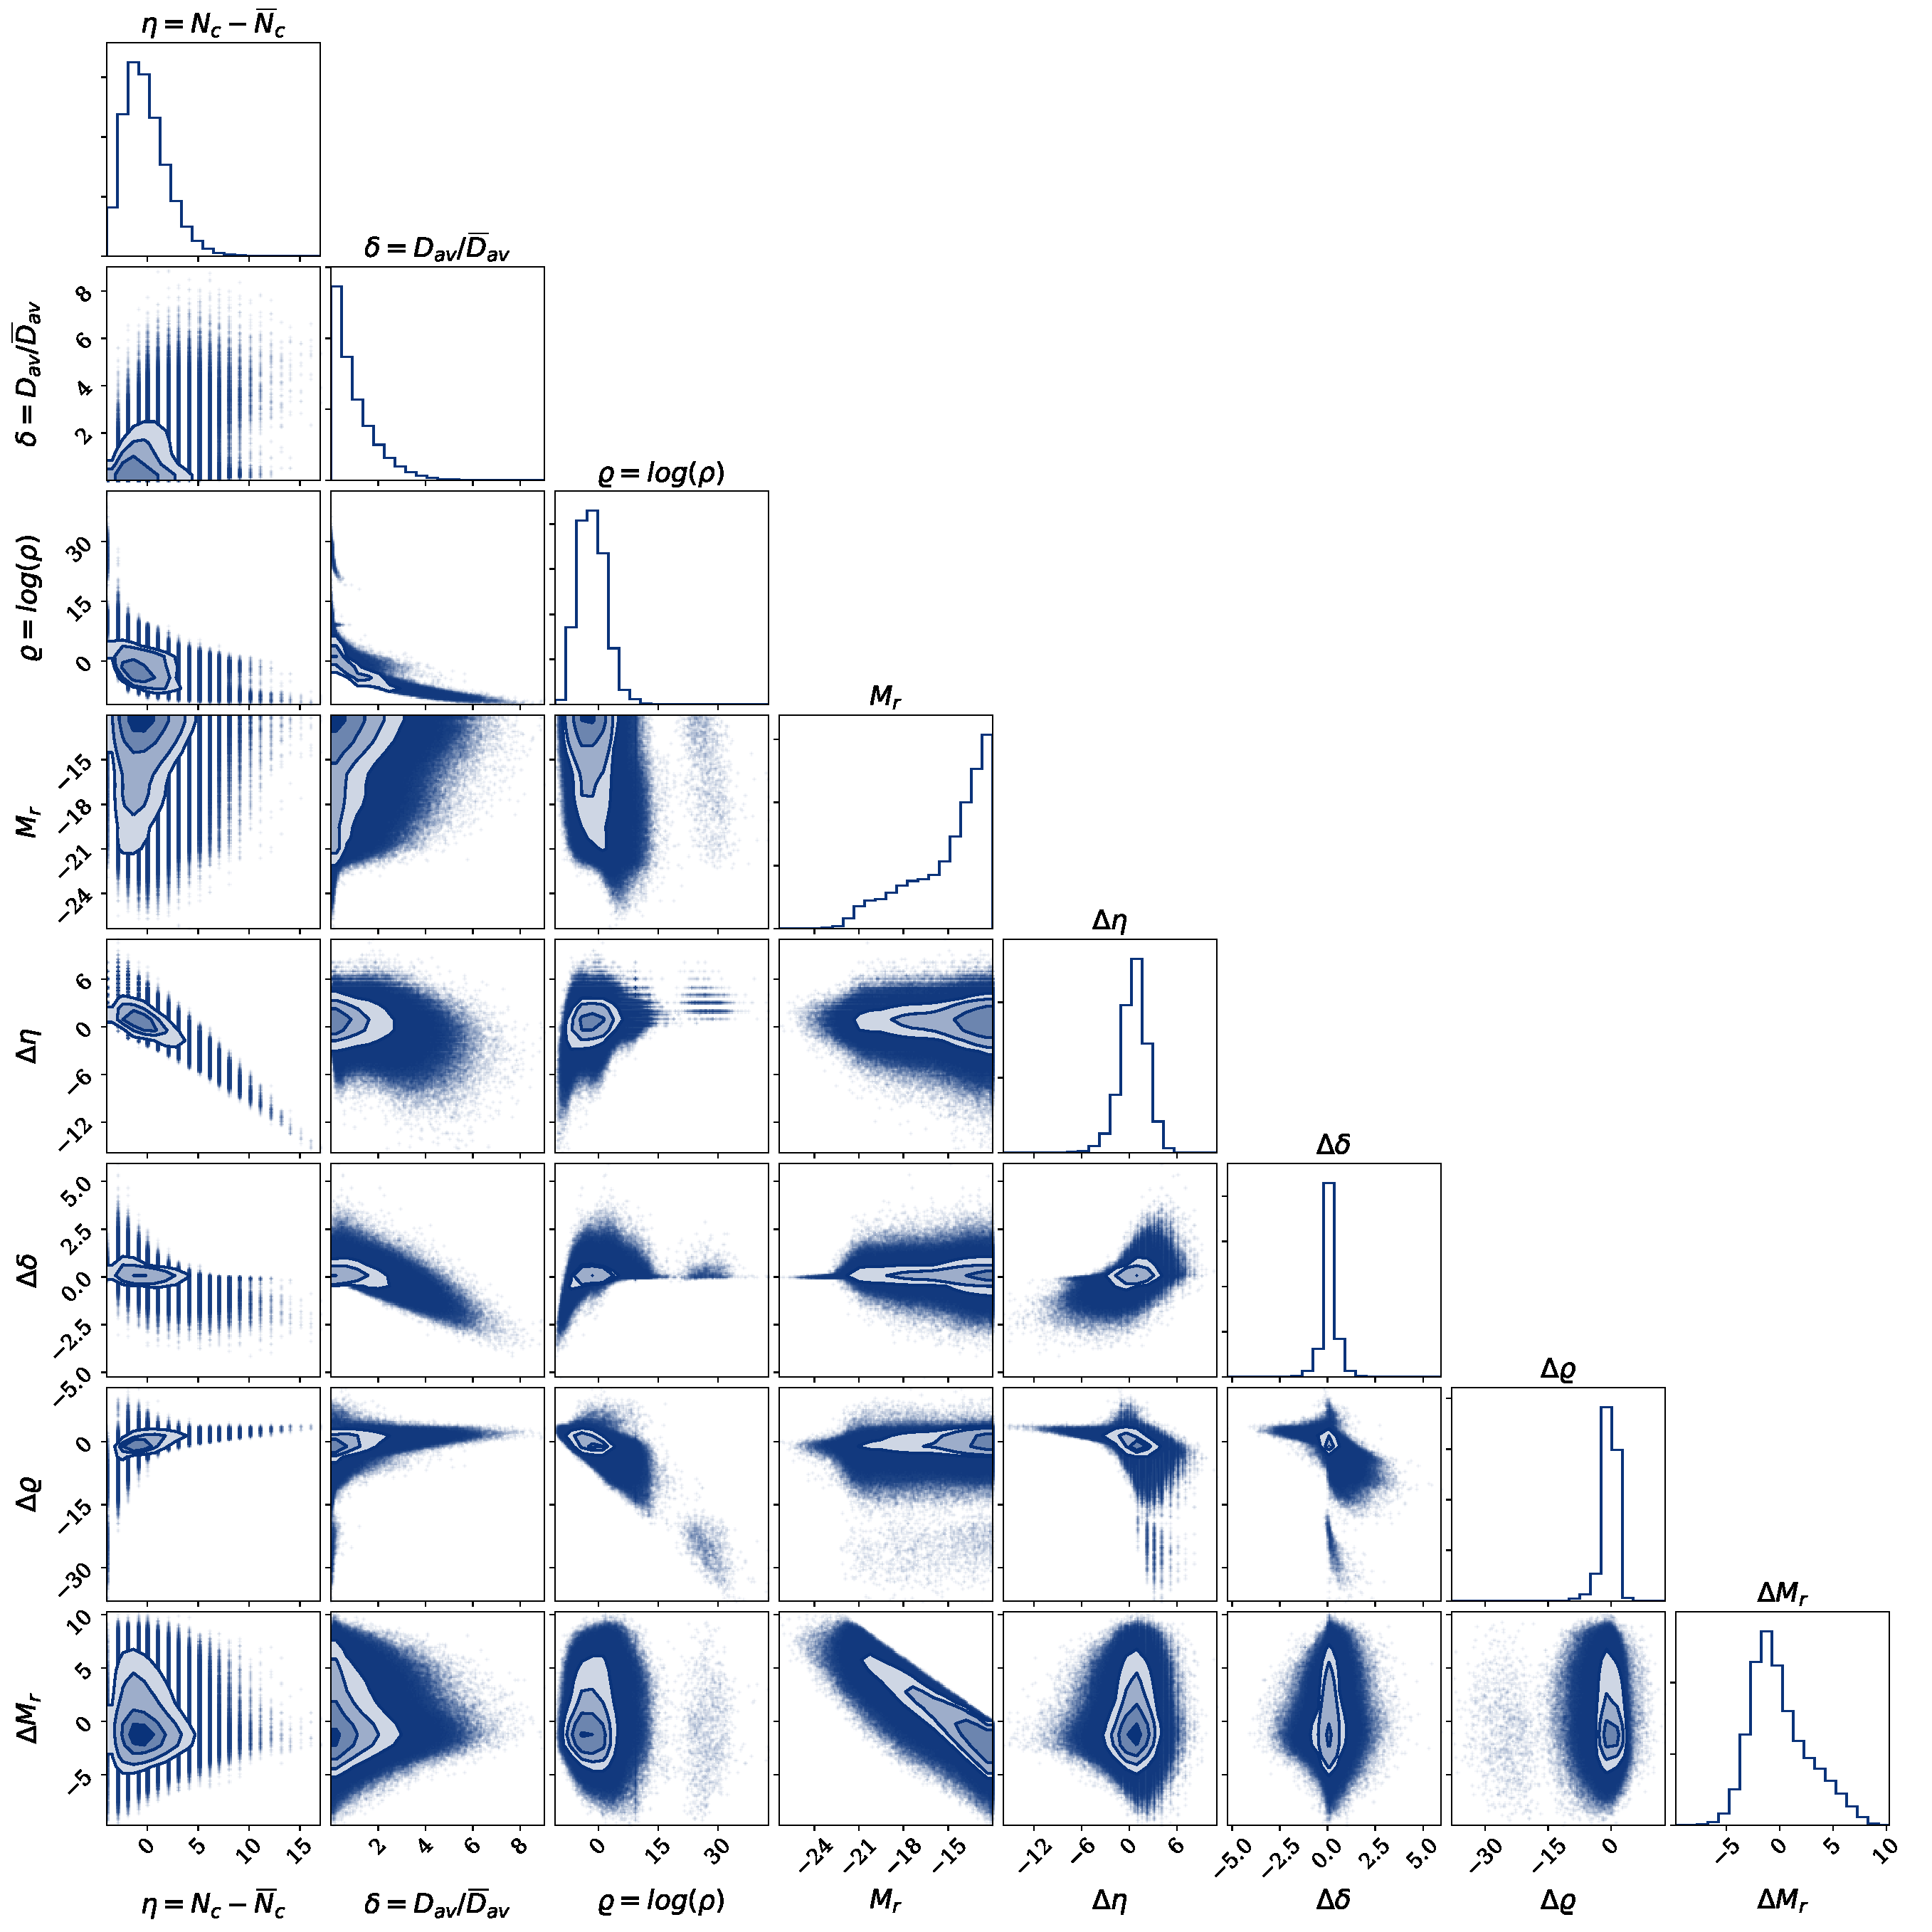
\includegraphics[scale=0.4]{Figs/p_all_features_correlations.pdf}
    \caption{Histograms and correlations curves for the eight features used to train the classifiers.}
    \label{fig:features}
\end{figure*}

\begin{figure*}
  \centering 
    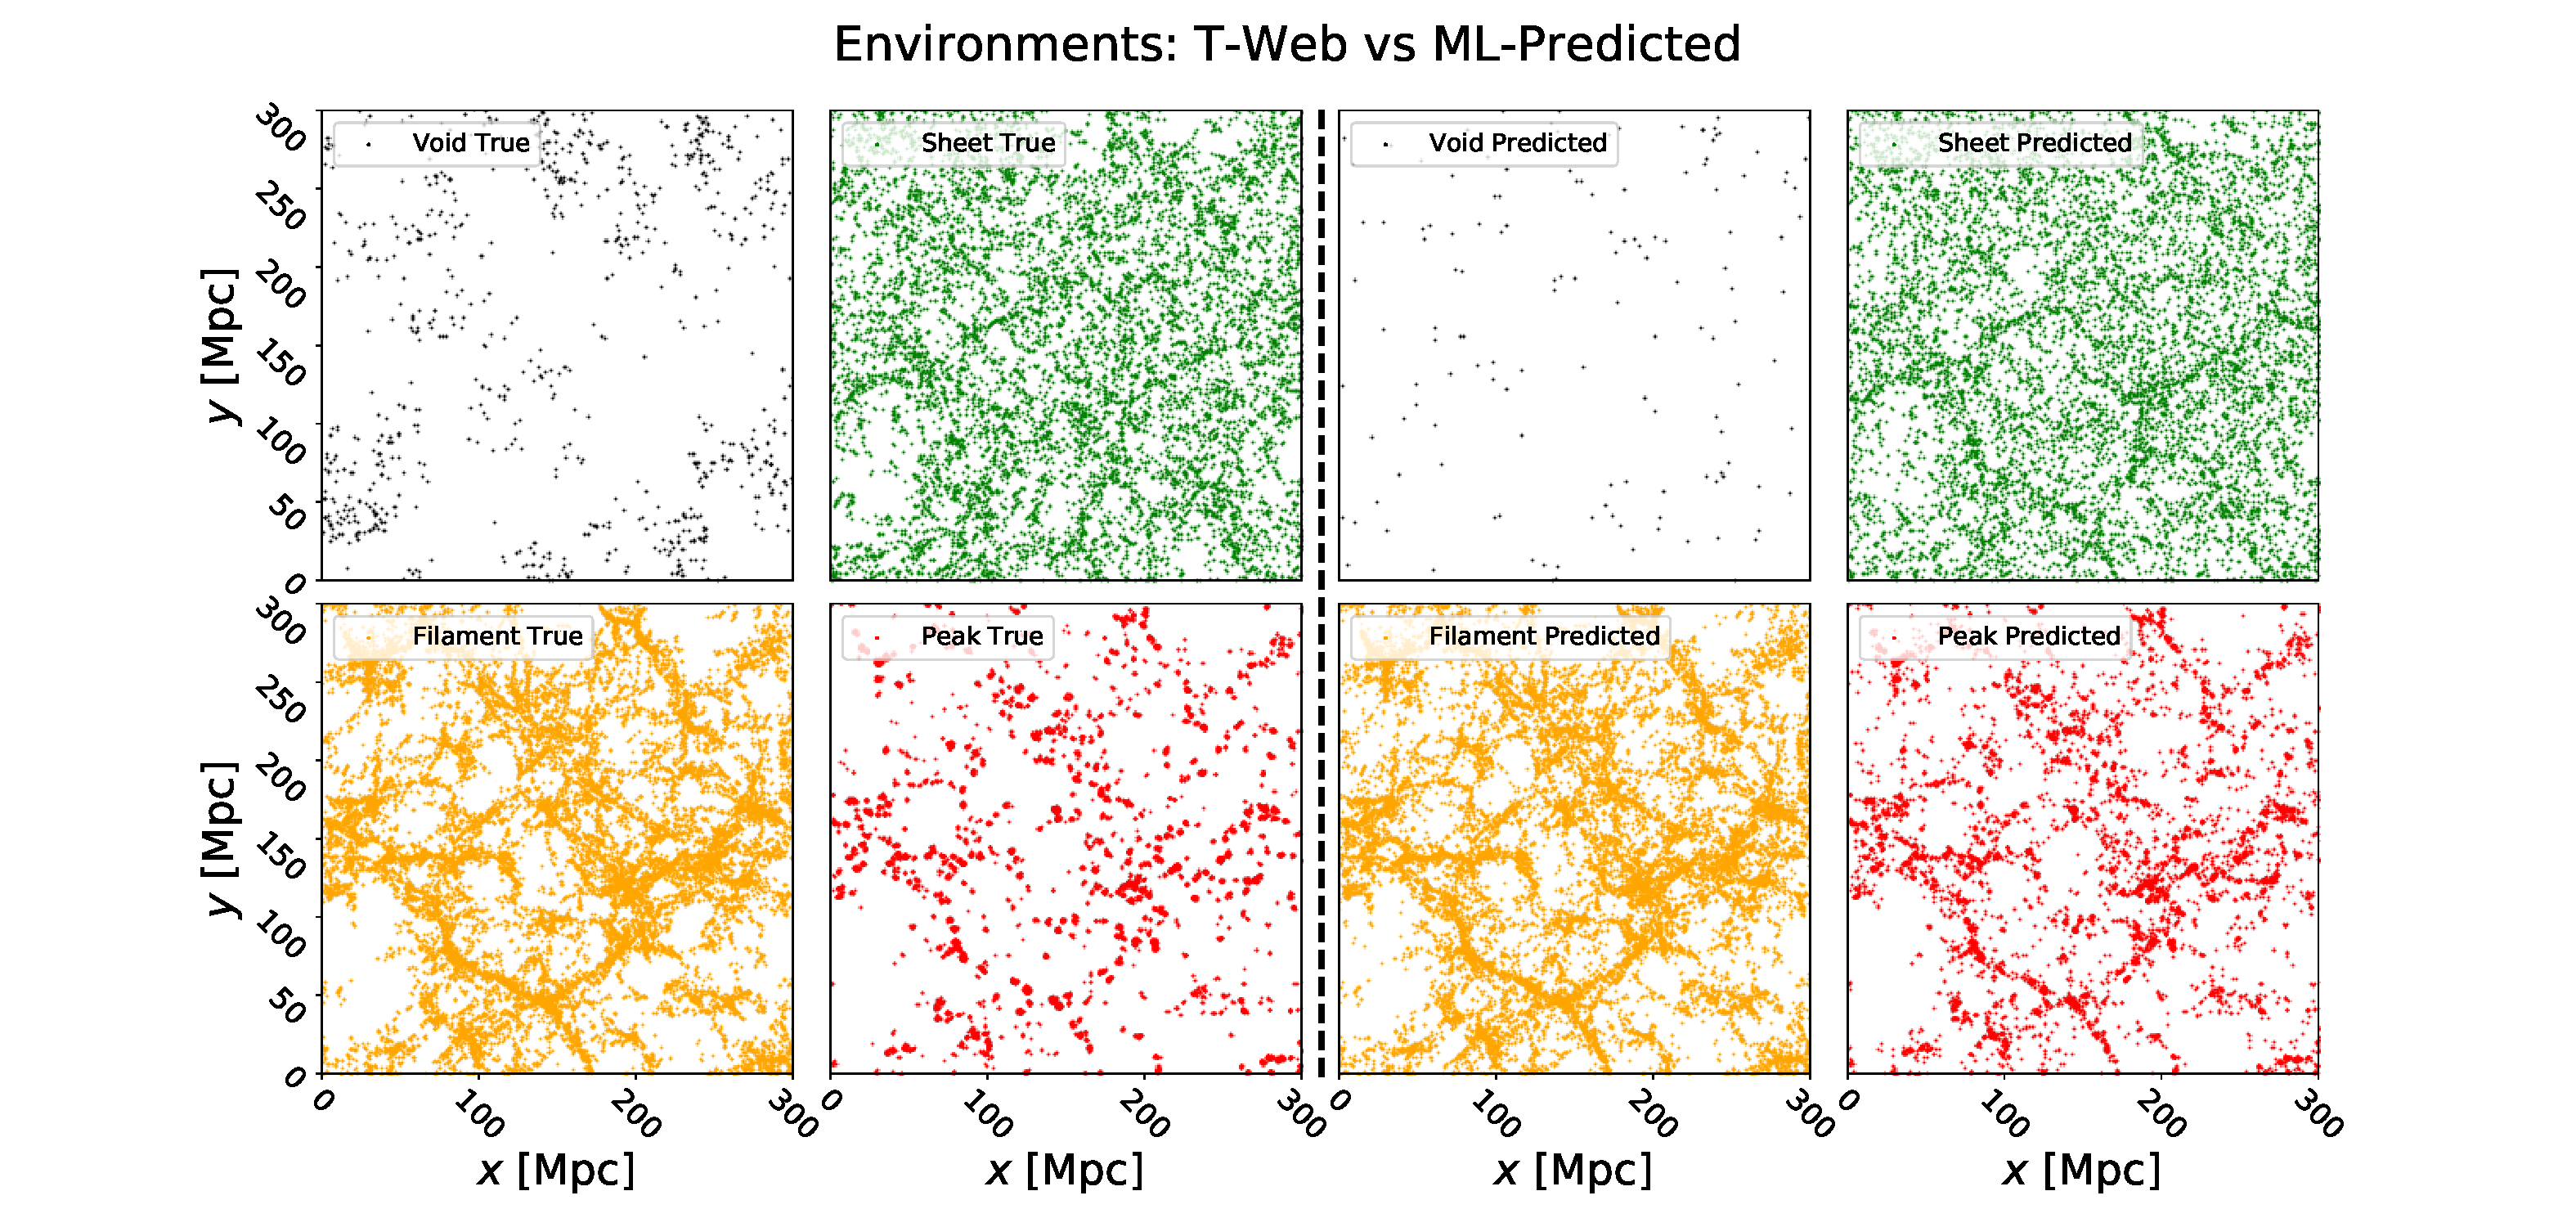
\includegraphics[scale=0.33]{Figs/Fig2.pdf}
    \caption{Comparison between the DM T-Web from the Illustris-TNG simulation and the environments predicted by the Tree Classifier algorithm}
    \label{fig:prediction}
\end{figure*}


\begin{figure}
\centering
    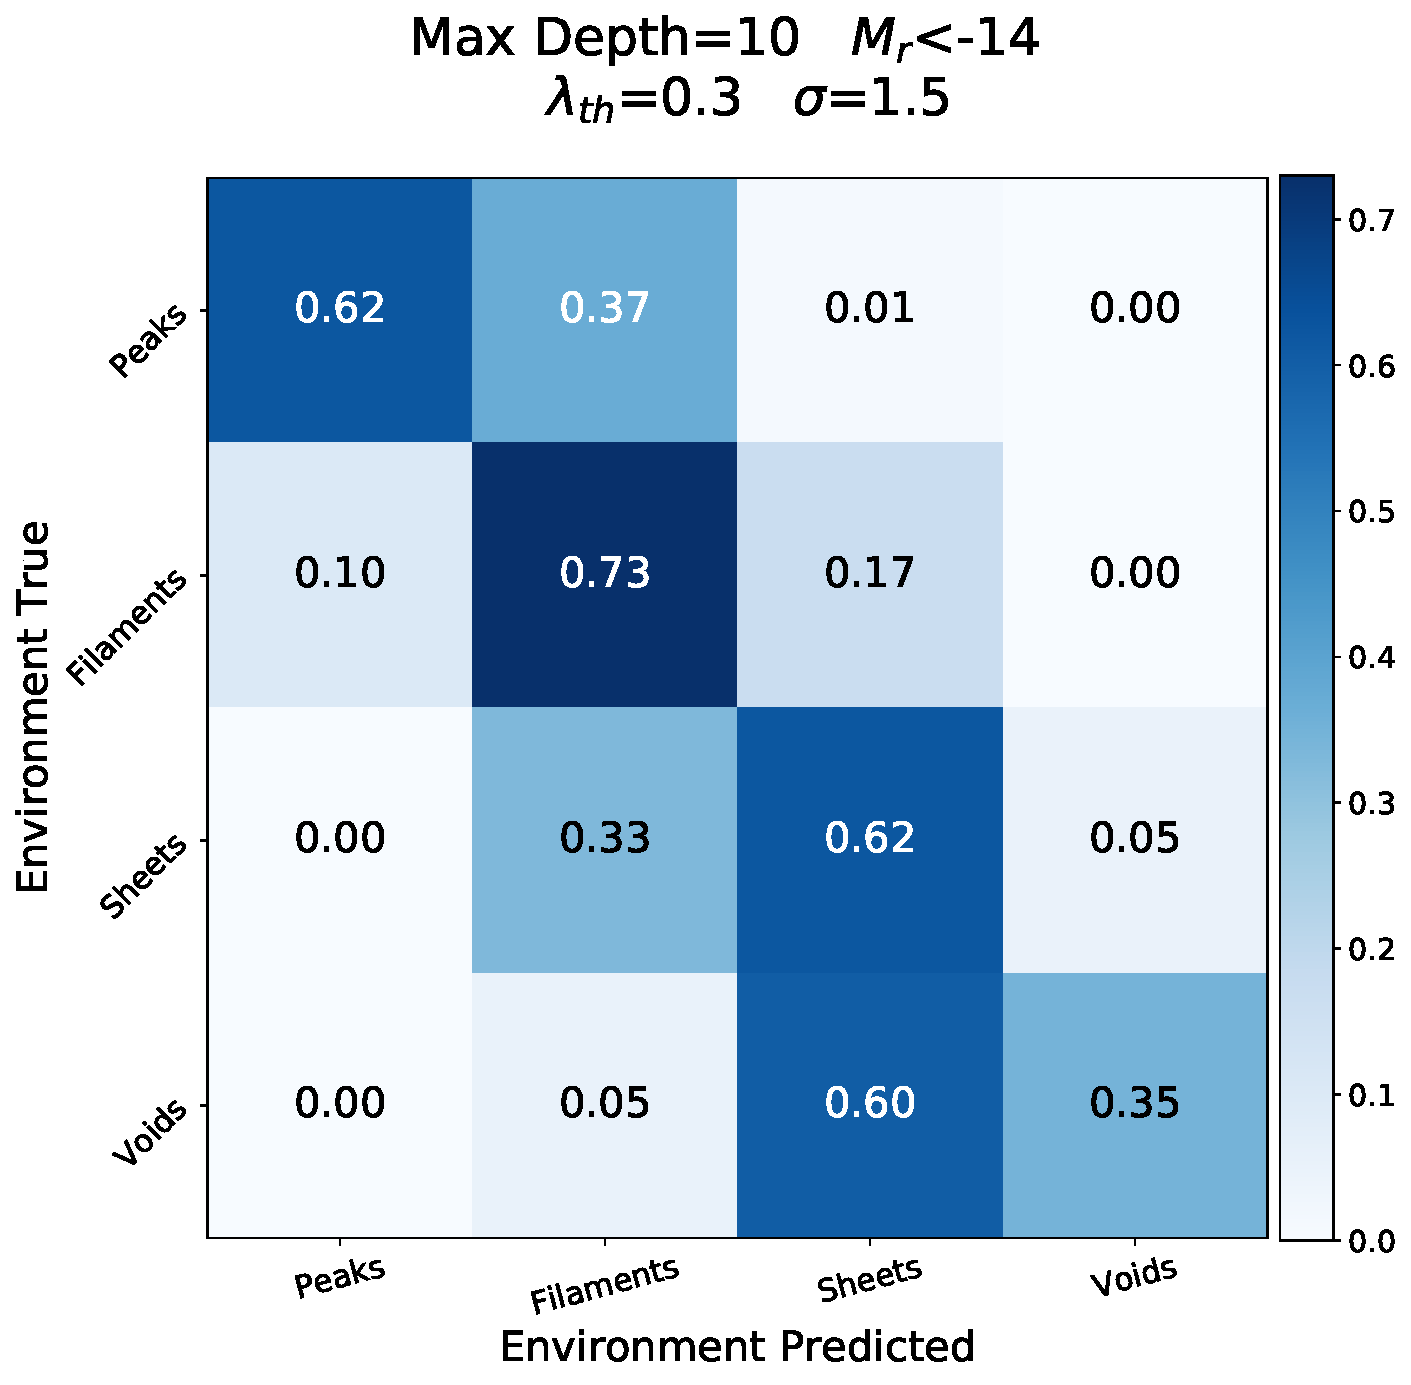
\includegraphics[scale=0.36]{Figs/p_CM_EnvPredTreeClass.pdf}
    \caption{Confusion Matrix for the best performing model with $\lambda_{th}$=0.3, $\sigma$=1.5 and $M_{r}<-14$. Columns represent the predictions, and rows the ground truth. In the CM for the prediction of peaks and sheets only the $62\%$ was predicted correctly. The best prediction are obtained for the filaments, where the $73\%$ was predicted correctly. The worst prediction was for the voids where only the $35\%$ was predicted correctly.}
    \label{fig:confusion_matrix}    
\end{figure}


\section{Linking the $\beta$-skeleton to the T-Web}\label{sec:link}

We use machine learning algorithms to predict the DM T-Web environment from features derived
from the $\beta$-skeleton.
We focus our work on a single snapshot at redshift $z=0$ without taking into
account Redshift Space Distortions.
In what follows we define the details of our setup for training and testing the algorithms.


\subsection{Features and meta-parameters}

We use eight features to train the classifiers.
Six features come from the $\beta$-skeleton algorithm applied over the distribution
of galaxies with $\beta=1$.
The first parameter is the number of connections minus the overall average number of
connections, $\eta = N_c - \bar{N}_c$. 
The second parameter is the ratio between the average distance across neighbors and its median
value over all galaxies in the simulations $\delta=D_{av}/\bar{D}_{av}$.
The third parameter is the logarithm of the pseudo-density $\rho$, $\varrho$. 
This pseudo density $\rho$ is defined as the inverse of the volume computed from the ellipsoid that best fits the distribution of graph neighbors.
We define three more features that we call $\Delta$-features: $\Delta\eta,\Delta\delta\,\text{and}\,\Delta\varrho$. 
These values are computed as the difference between the corresponding value in a node and the 
average value over first neighbors nodes.
Two more features come from the simulation. The absolute magnitude in the 
$r$-band, $M_r$, and its corresponding $\Delta M_r$.
Figure \ref{fig:features} shows the histogram for all $\beta$-skeleton features.



We also use the threshold $\lambda_{th}$ and the smoothing parameter $\sigma$ as
meta-parameters that drive the T-Web classification. 
We take $\lambda_{th}=0.0, 0.1, 0.2, 0.3, 0.4$ and $0.5$.
For the smoothing parameter we take the values $\sigma=0.5$, $1.0$, $1.5$, $2.0$ and $2.5$. 

\subsection{Classification Algorithms}

We applied three different supervised machine learning algorithms: support vector machine (SVM),
classification trees and random forests as implemented in scikit-learn. 
 For each algorithm we explore the following metaparameters:
\begin{itemize}
    \item SVM: 
        \begin{itemize}
            \item $kernel$: \textit{rbf} or Radial basis function
            \item $max\_iter$= 500,1000,1500,2000,2500.
        \end{itemize}
    \item Classification trees
        \begin{itemize}
            \item \textit{Max depth}: From 1 to 30.
        \end{itemize}
    \item Random forest
        \begin{itemize}
            \item \textit{Max depth}: 10.
            \item \textit{Number of estimators}: From 1 to 100.
        \end{itemize}
\end{itemize}


\subsection{Model evaluation}

From the box simulation, we select randomly a 50$\%$ of galaxies by class of environment to train the ML algorithms. We use the other 30$\%$ as test and  20$\%$ as validation. Due the box simulation has periodic conditions, we selected the galaxies located between 5Mpc and 295Mpc in order to make the model consistent.  
As success metrics, we compute the precision, recall, gain (the rate between the true positives
and the total predictions) and the F1 score (harmonic mean between precision and recall).
We use the average F1 score across classes to select the best models and its meta-parameters.

\begin{figure*}
    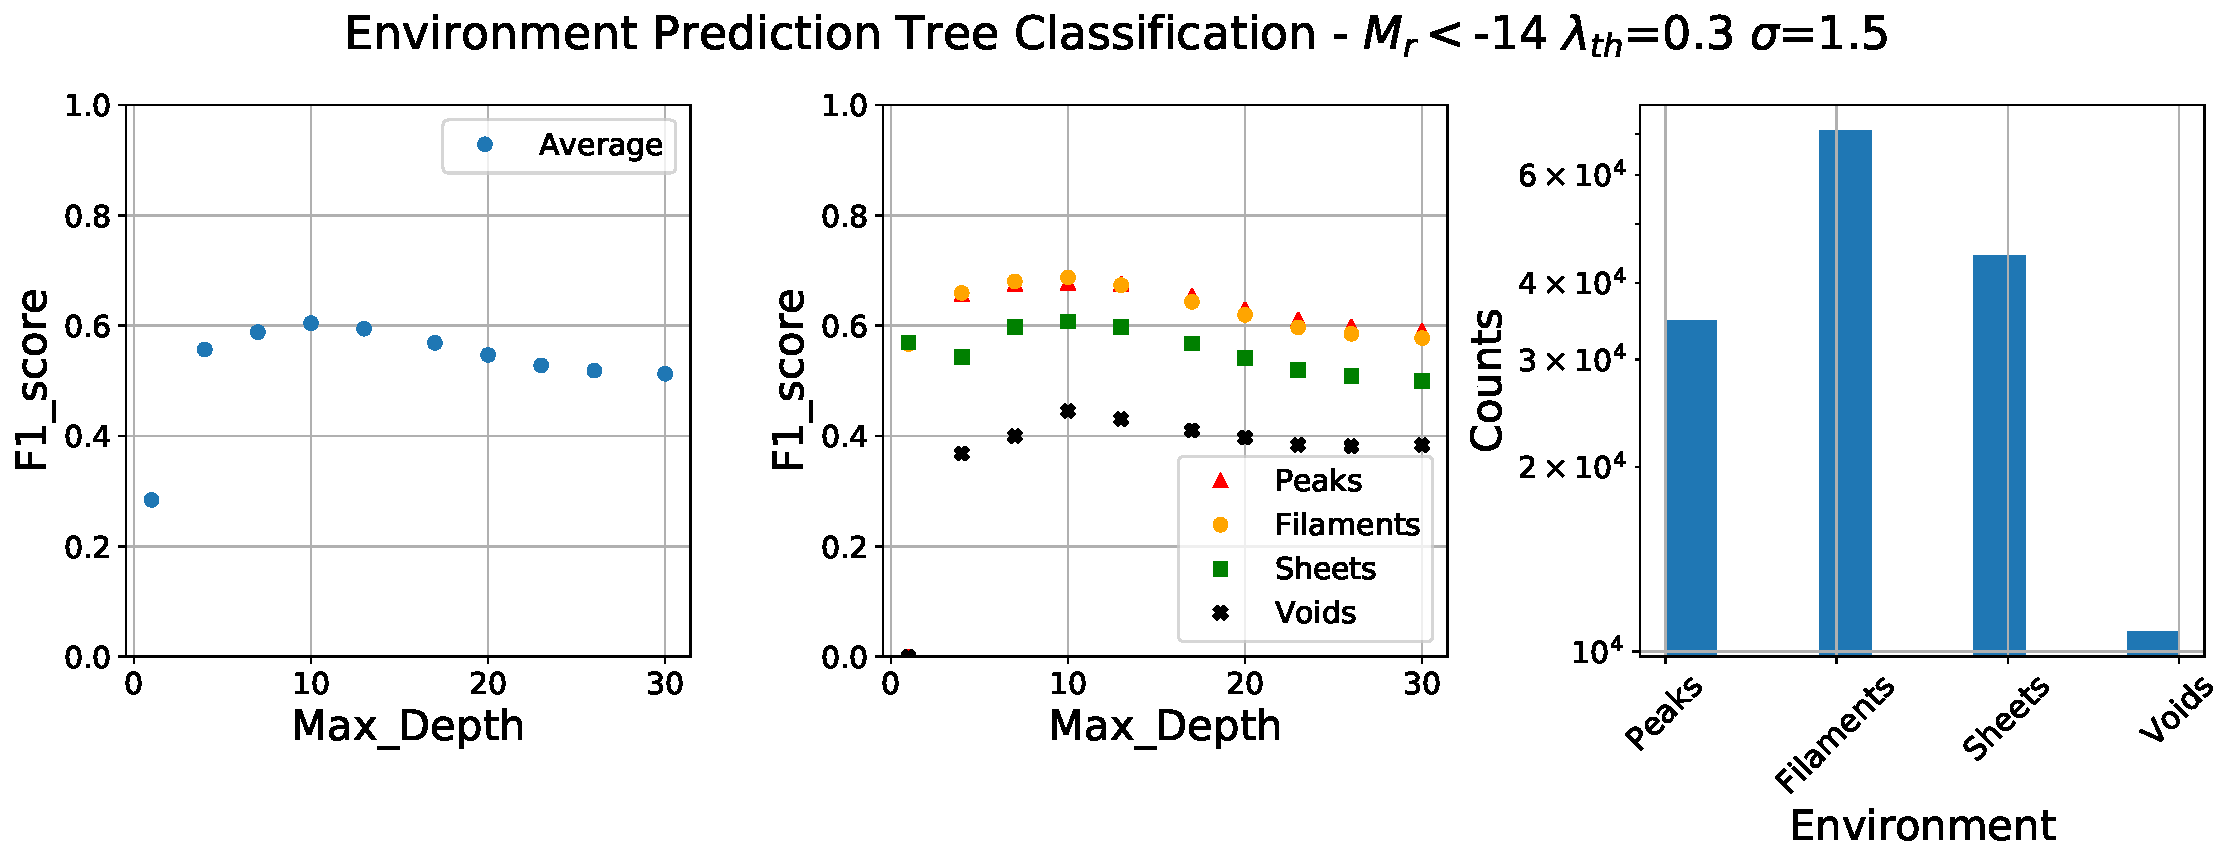
\includegraphics[scale=0.45]{Figs/p_F1_EnvPredTreeClass.pdf}
    \caption{The evaluation of the classification tree algorithm was computed with the F1 score. Here the evaluation of the F1$_{av}$ score was computed for $\lambda_{th}=0.3$, $\sigma=1.5$ and $M_r<-14$.  In the left figure was evaluated the F1$_{av}$ score for the prediction of all environments as a function of the Max Depth of the classification tree. The center figure show us the evaluation for the prediction by environment, here the best predicted environment are the filaments, for this, the maximum F1 score is near to 0.8. The right figure show the population by environment using to make the prediction with the Tree Classification ML algorithm.}
    \label{fig:F1_curve}
\end{figure*}


\begin{figure*}
\centering
    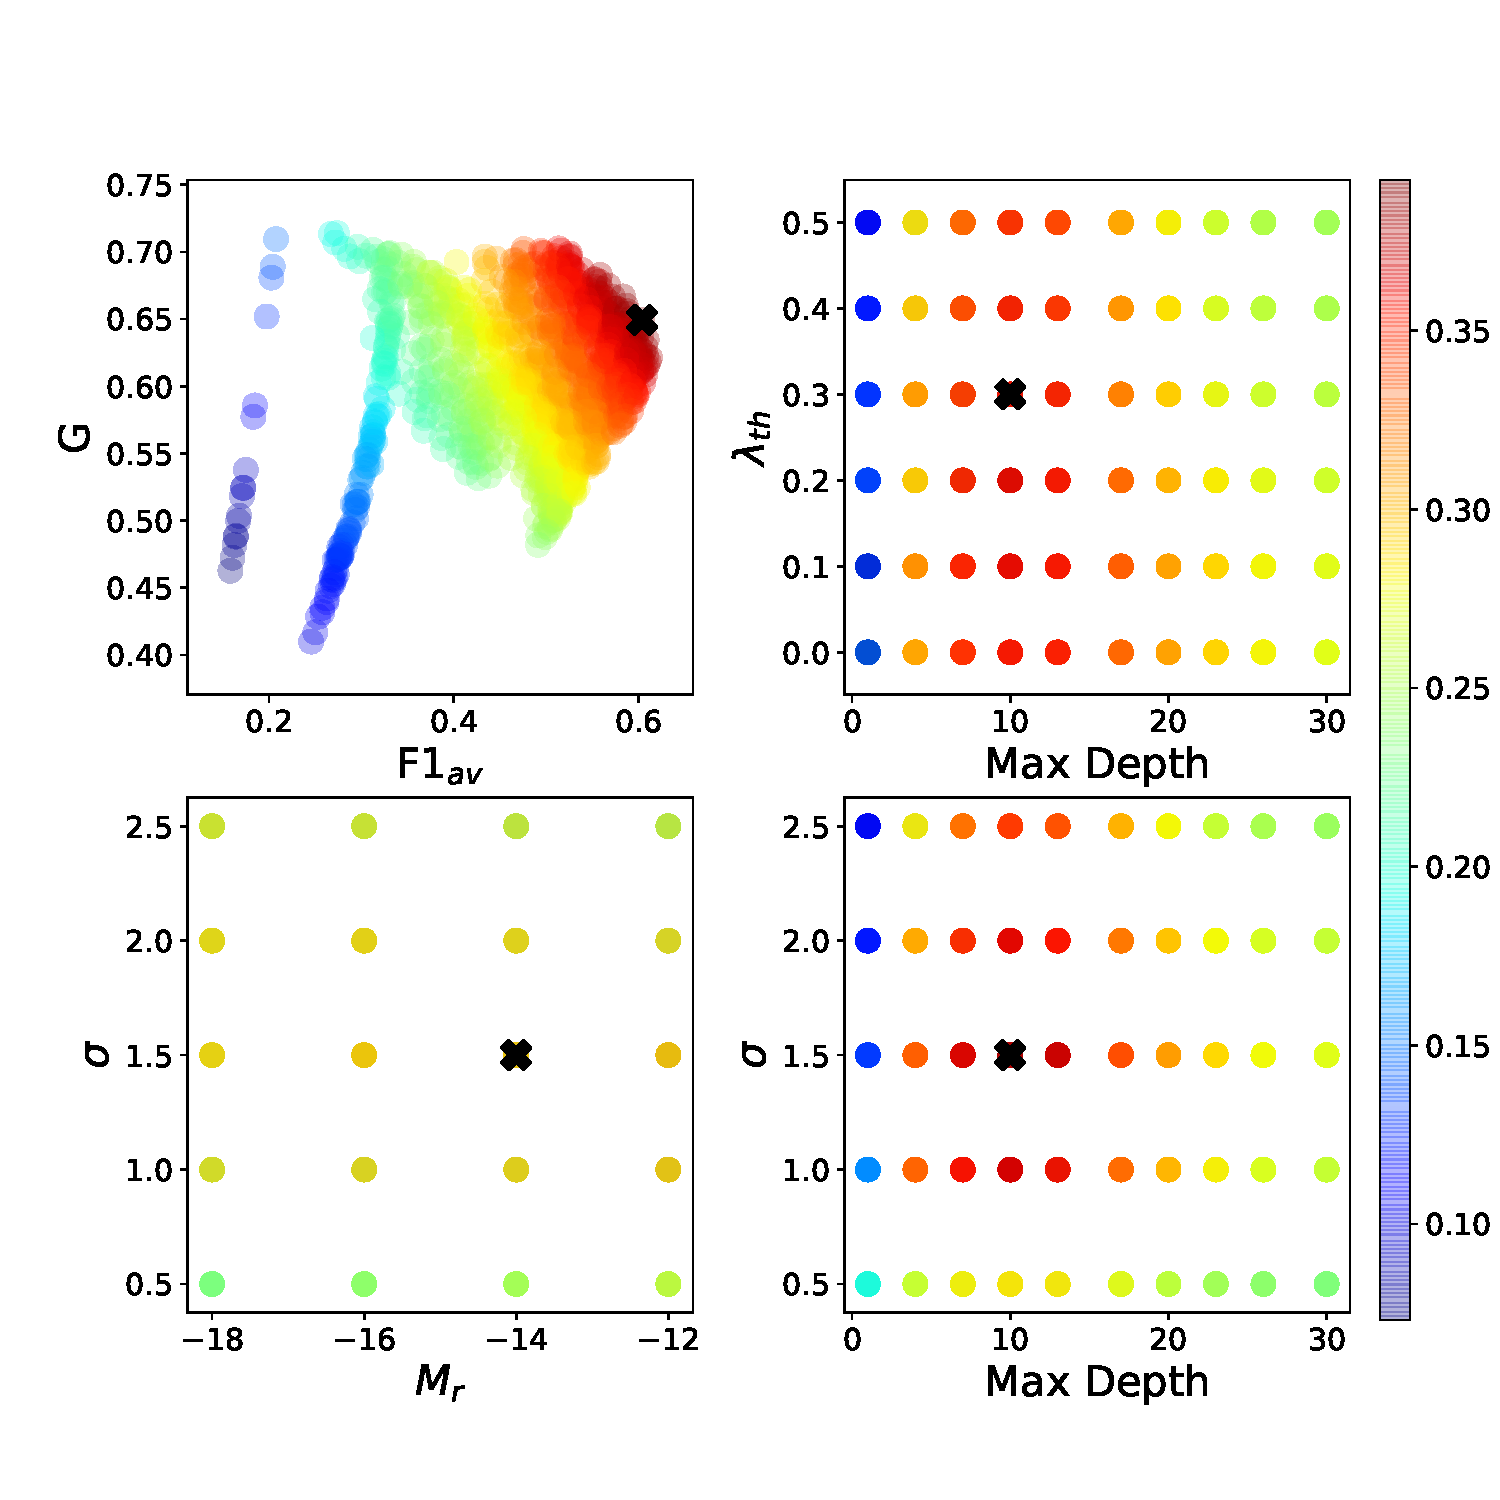
\includegraphics[scale=0.5]{Figs/p_FS_Tree.pdf}
    \caption{Plots for the analysis of the features space. Here we found the best configuration of the features to maximize the Gain and the $F1$ average score. The values founded over the features that maximize both scores are $\lambda_{th}=0.3$ ,$\sigma=1.5$, $M_{r}<-14$ and Max Depth=10. The colors in the left bottom figure are the product between the Gain and the $F1$ average, this scale varies between 0 and 1.}
    \label{fig:features_space}
\end{figure*}


\section{Results}\label{sec:results}

A comparison between the best results for the machine learning methods used are resumed in the Table \ref{tab:methods}. Figure \ref{fig:prediction} shows the comparison between the ground truth environments (left) and the prediction by the best ML algorithm with the optimized parameters and meta-parameters (right). 
The visual impression is that the sheets and filaments have good predictions, 
peaks are reasonable, while voids are the worst.

\begin{table}
\centering
\begin{tabular}{l|l|l|l|l|l|}
 F1 & Peaks & Filaments & Sheets & Voids & Average \\ \hline
\multicolumn{1}{|l|}{SVM} & 0.000 & 0.000 & 0.687 & 0.617 & 0.326 \\ \hline
\multicolumn{1}{|l|}{R. Forest} & 0.682 & 0.693 & 0.602 & 0.397 & 0.594 \\ \hline
\multicolumn{1}{|l|}{Trees} & 0.678 & 0.687 & 0.608 & 0.445 & 0.605 \\ \hline
\end{tabular}
\caption{F1 score by environment and average. Comparison between the three supervised machine learning methods, SVM has the worst F1 average score, the best F1 average score is for the tree classifier.}
\label{tab:methods}
\end{table}

This visual impression is confirmed by the quantitative results shown in Figure \ref{fig:confusion_matrix}.
We observe that the best prediction is for filaments where the $73\%$ of the true galaxies in filaments are correctly predicted. 
This fraction is followed by $62\%$ of correct peaks and sheets galaxies with
a low value of $35\%$ void galaxies classified correctly.


The classification trees have other types of configurable parameters, the most common parameter is the depth of the branches in the tree, we evaluate the classification tree with the F1 score as a function of the max depth parameter. 
Figs.\ref{fig:F1_curve} show the behavior of the F1 score as a function of the max depth in the tree in contrast to the populations of the environments, the left figure shows the F1 average score, the maximum is near to 0.6 for a max depth equal to 10. 
The center figure shows the F1 score for the four environments, the best environment predicted was the filaments followed by the peaks and sheets, the worst predicted environment was the voids, this due the population of them as we can see in the right figure of the Fig.\ref{fig:F1_curve}, we can observe that the amount of voids is considerably less than the others environments almost in one order.

In order to select the best set of features we evaluated the classification tree for different ranges of the features and select the values that maximize simultaneously the F1 average score and the gain. Fig.\ref{fig:features_space} shows the ranges probed for the features. 
The colors in the figure F1$_{av}$ vs. gain (G) are the product between them, this product varies between 0 and 1. 
The maximum value for this product was indicated with a black cross and indicates the best set of values for the parameters of the features space. 
The values obtained for the parameters are $\lambda_{th}$=0.3, $\sigma$=1.5, \textit{max depth}=10 and $M_r<$-14.
The values in the range of $M_r$ are related to cuts in the luminosity. The classification tree was training with different volumes of galaxies that depended on these cuts in luminosity. Another mechanism to select the best meta-parameters was computed the area under the precision-recall curve, however this information was not clear due the noise in the curve. So, this score was ignored to select the best meta-parameters.

Fig.~\ref{fig:feature_importance} shows the importance of the features for classification trees. The most important feature for our model is the $\Delta \delta$ feature related to the local average distance between connections, followed by the average distance between connections $\delta$. This shows us that the separation between the galaxies is a parameter that can determinate the T-Web environment for a galaxy. The number of connections is not a relevant parameter to determine the environment due to its importance is not significant.

The same evaluation over the features space with the classification trees was made with the SVM and random forest. The values for the parameters that maximize the F1 average score and the gain were $\lambda_{th}=0.2$ ,$\sigma=2$ and $M_{r}<-18$ for the SVM and $\lambda_{th}=0.3$ ,$\sigma=1.5$ and $M_{r}<-14$ for the random forest. The SVM algorithm was trained with the robust bias function (rbf) kernel, the best value obtained for the F1 average score was 0.326, worst than the tree classifier. In the random forest case, we could optimize the prediction with the number of estimators fixing the max depth for the trees in 10, the results showed that the max value obtained for the F1 average score was near to 0.594 with a number of estimators equal to 20. These evaluations confirmed that the tree classifier is the best algorithm to reconstruct the T-Web.

The best model was evaluated including the information of the features extracted from the 2 and 3-skeleton, the results do not vary in comparison when we used only the features of the 1-skeleton, these showed that the 2 and 3-skeleton do not contain important information to predict the T-Web.

\begin{figure}
\centering
    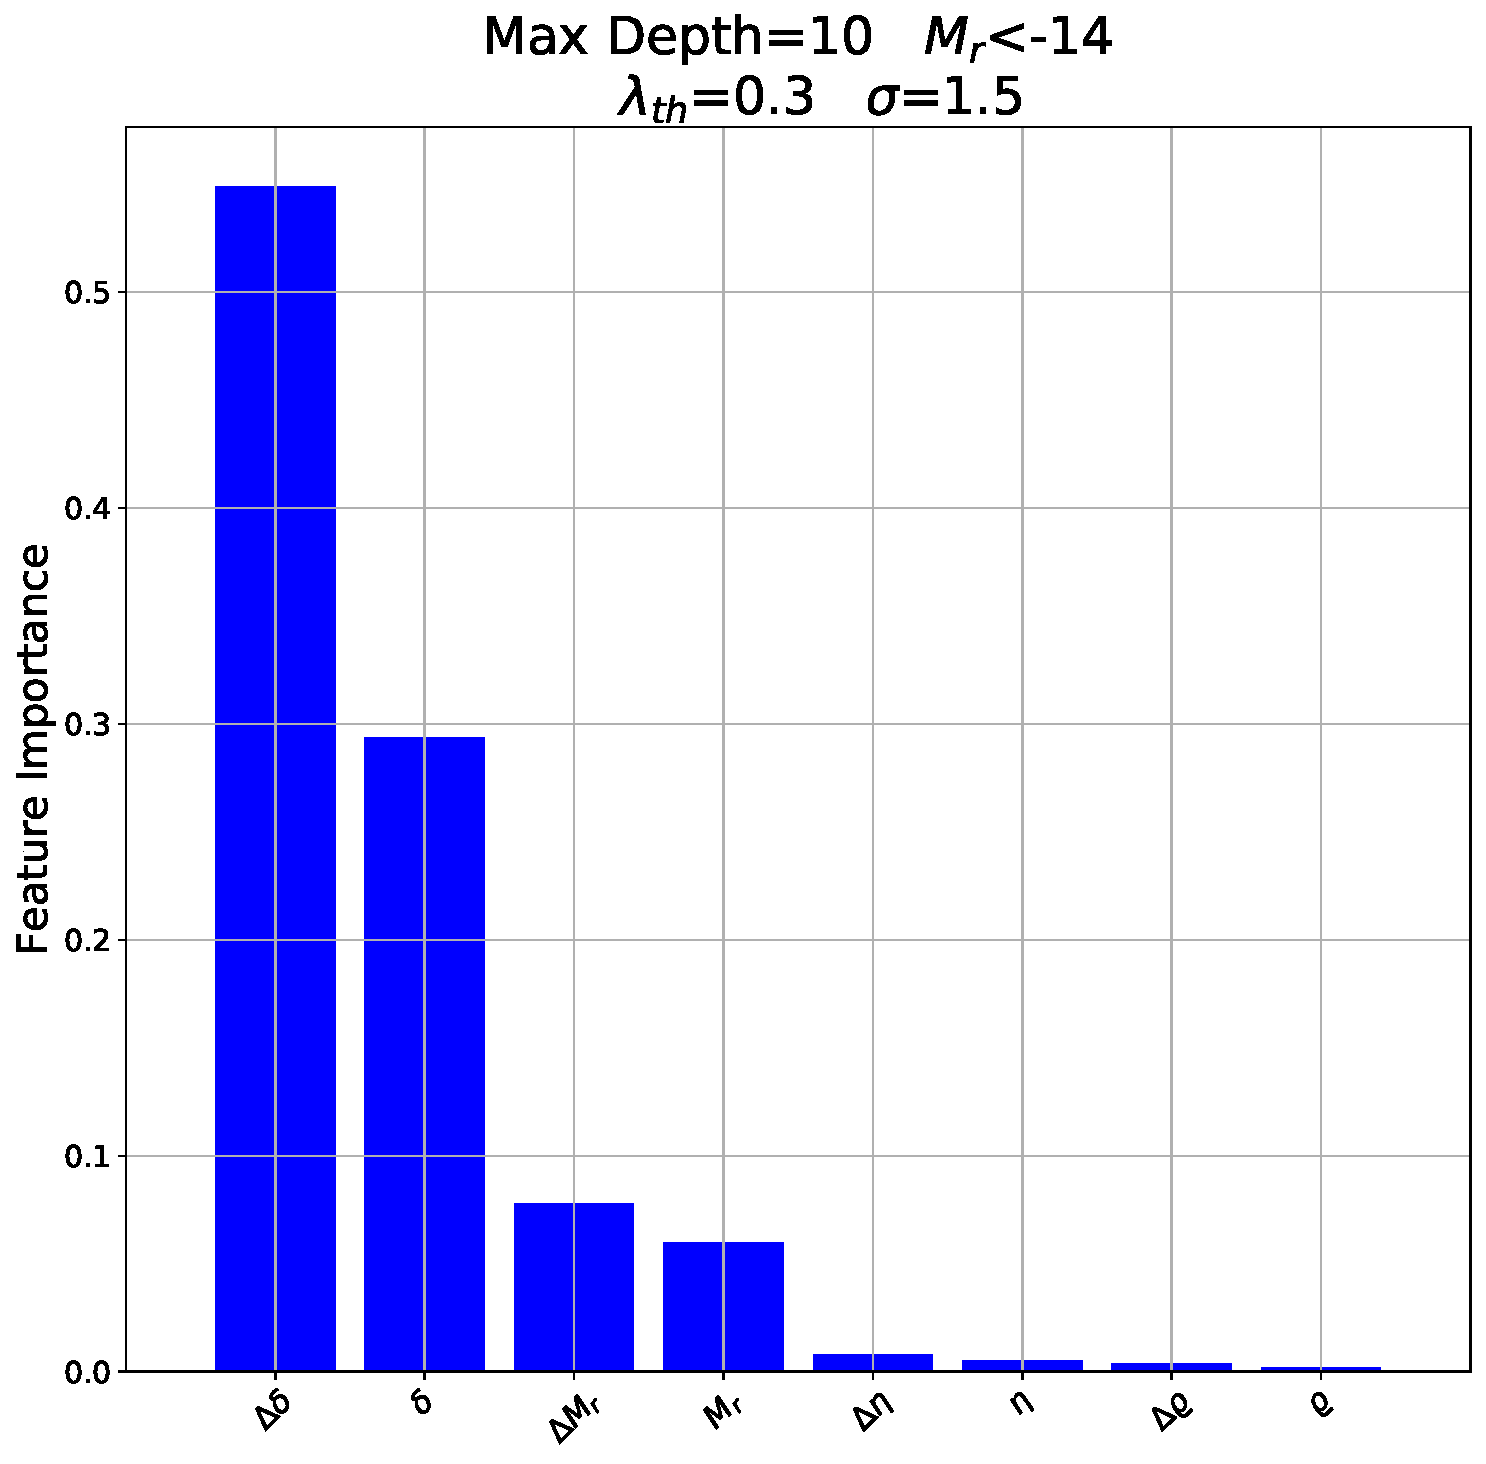
\includegraphics[scale=0.32]{Figs/p_FI_EnvPredTreeClass.pdf}  
    \caption{Feature importance for the best classification with $\lambda_{th}$=0.3 ,$\sigma$=1.5, $M_{r}<-14$ and Max Depth=10. This figure show us that the most important variable from the $\beta$-skeleton to make the best prediction are related with the average distance between the connections of the galaxies. The importance of the $\delta$ parameter is near to the $50\%$.}
    \label{fig:feature_importance}     
\end{figure}

\section{Conclusions}\label{sec:conclusions}

In this paper we presented a method to predict the dark matter cosmic web
environment of a galaxy from its neighbor graph information.
We used the T-web as the cosmic web definition \citep{Forero-Romero2009}
and the $\beta$-skeleton graph \citep{Fang2019} 
to describe the relative spatial distribution of the galaxies. 
The link between the T-web and the graph is done through different
machine learning algorithms: support vector machines, random forests and
classification trees.

We test the method using data from the Illustris-TNG simulation.
The T-web is calculated on a grid of cell size $0.8$\Mpch 
and a Gaussian smoothing scale $\sigma$ and an eigenvalue threshold $\lambda_{th}$.
The $\beta$-skeleton is computed over galaxies brighter than 
an $r$-band absolute magnitude cut $M_{r}$.
For each simulated galaxy we build the $\beta$-skeleton and
compute features such as the number of connections, the average connection
length, the pseudo-density and the difference of these quantities with
respect to the average over first-neighbors.

We find that the T-web environment that is best predicted has smoothing
scale of $\approx1.5$ \Mpch and an threshold $\lambda_{th}=0.3$. 
This turns out to be the ballpark range  favored in previous publications
for T-web  studies for the resulting classification to match the visual impression of the cosmic web \citep{Forero-Romero2009}.
We also find that the features computed with the $1$-skeleton 
(Gabriel Graph) are enough to obtain good predictions. 
The best classification results are not sensitive to the $r$-band
magnitude cut, although a cut of $M_r>-14$ gives the best results.

The best algorithm to predict the environment are the classification
trees followed closely by random forests. 
Support Vector Machines provide the worst results.
From the classification trees we are able to determine that the two most
important features for the environment classification are the average
connection length over the neighbors and the difference of this quantity
with respect to the average over its first neighbors.

The environments that are best predicted are in decreasing order: 
filaments, peaks, sheets and voids. 
This ranking follows the number of galaxies found in each of these environments.
Galaxies in voids represent less that $2\%$ of the total number of galaxies and 
are the hardest class to predict, with $F1$-scores of $\approx0.2$.
Motivated by this limitation, in future work we will present a method to define
voids from the $\beta$-skeleton graph.

All the results we reported here were obtained using a single snapshot at a 
redshift $z=0$.
Our results provide the baseline for future work that will have to quantify 
the effect of redshift space distortions and survey incompleteness in order to
predict  the DM T-Web form survey data.
Nevertheless, the two most interesting features of our method are: a) it does not
rely either on binning the galaxy data on a grid and b) it does not require 
a dark matter density reconstruction.



\section*{Acknowledgements}
\textcolor{red}{Faculty}\\
We are thankful to the community developing and maintaining open source packages fundamental to our work: numpy
\&  scipy  (Walt  et  al.  2011),  the  Jupyter  notebook  (P\'erez \& Granger 2007; Kluyver et al. 2016), matplotlib (Hunter2007) and  scikit-learn (Pedregosa et al. 2011).
%%%%%%%%%%%%%%%%%%%%%%%%%%%%%%%%%%%%%%%%%%%%%%%%%%

%%%%%%%%%%%%%%%%%%%% REFERENCES %%%%%%%%%%%%%%%%%%
% The best way to enter references is to use BibTeX:
\bibliographystyle{mnras}
\bibliography{references}

% Alternatively you could enter them by hand, like this:
% This method is tedious and prone to error if you have lots of references
%\begin{thebibliography}{99}
%\end{thebibliography}
%%%%%%%%%%%%%%%%%%%%%%%%%%%%%%%%%%%%%%%%%%%%%%%%%%

%%%%%%%%%%%%%%%%% APPENDICES %%%%%%%%%%%%%%%%%%%%%
%\appendix
%\section{Some extra material}
%%%%%%%%%%%%%%%%%%%%%%%%%%%%%%%%%%%%%%%%%%%%%%%%%%

% Don't change these lines
\bsp	% typesetting comment
\label{lastpage}
\end{document}
% End of mnras_template.tex
